\setcounter{chapter}{0}
\chapter{Basic Topology}

\setcounter{section}{0}
\section{Set}

\begin{notation}
    \begin{itemize} ~
        \item $\mathbb{N}_{n} = \{ 1,2,\cdots ,n \}$
        \item $A^{n} = \{ (a_1,\cdots ,a_n):a_i \in A \}$
    \end{itemize}
\end{notation}

\begin{definition}[Finite; Countable] Let $A$ be a set.
    \begin{itemize}
        \item $A$ is \textit{finite} if $A \sim \mathbb{N}_{n}$ for some $n$.
        \item $A$ is \textit{countable} if $A \sim \mathbb{N}$ or $A$ is finite.
        \item $A$ is \textit{infinite} if $A$ is not finite.
        \item $A$ is \textit{uncountable} if $A$ is not countable.
        \item *$A$ is \textit{infinite} if $\exists B \subset A$, $A \sim B$
    \end{itemize}
\end{definition}

\begin{definition}[Cardinality] Sets $A,B$ have the same \textit{Cardinality} denoted $A \sim B$ if there is a bijection $f:A \to B$.
\end{definition}

\begin{remark}
The relation $\sim $ defined in Definition 2 is equivalent.
\end{remark}

\begin{definition}[Sequence] \textit{A sequence $\{ x_n \}$ in $X$} is $f: \mathbb{N} \to X$, where:
    \begin{itemize}
        \item $x_n \in X$, $n \in \mathbb{N}$
        \item $f(n) = x_n$
    \end{itemize}
\end{definition}

\begin{prop} Every subset of a countable set is countable.
    \\ (No uncountable set can be subset of a countable set)
\end{prop}
\begin{proof}
Let $A$ be a countable set,
\\If $E \subset A$ is finite, then countable.
\\If $E \subset A$ is infinite, then we construct a sequence to obtain a 1-1 correspondence between $J$ and $E$.
\end{proof}

\begin{lemma} ~
    \begin{itemize}
        \item If $\exists f: \mathbb{N}\to S$ that is subjection, then $S$ is countable.
        \item If $\exists g: S\to \mathbb{N}$ that is injection, then $S$ is countable. 
    \end{itemize}
\end{lemma}

\begin{prop} Let $\{ E_n : n \in \mathbb{N}\}$ be a countable collection of countable sets. \\
    Then $$
    \bigcup_{n = 1}^{\infty}E_n
    $$
is countable.
\end{prop}

\begin{prop}Let $A$ be a countable set, then $A^{n}$ is countable.
\end{prop}
\begin{corollary}
The set of all rational numbers is countable.
\end{corollary}

\begin{prop}Let $A$ be the set of all sequence $\{ x_n \}$ in $\{ 0,1 \}$, then $A$ is uncountable.
\end{prop}

\begin{corollary} ~
\begin{itemize}
    \item $\mathcal{P}(\mathbb{N})$ is uncountable.
    \item $\mathbb{R}$ is uncountable.
\end{itemize}
\end{corollary}

\section{Metric space}
\begin{definition}[Metric space; Points; Distance] Let $X$ be a set. $X$ is a metric space if:
    \\$\exists d:X\times X \to \mathbb{R}$ such that $\forall p,q \in X$:
    \begin{itemize}
        \item $d(p,q)>0$ if $p\neq q$; \\$d(p,p) = 0$
        \item $d(p,q) = d(q,p)$
        \item $d(p,q)\le d(p,r)+d(r,q)$, $\forall r \in X$
    \end{itemize}
    where $p,q$ are called \textit{points}, and $d$ is called a \textit{distence function}.
\end{definition}

\begin{remark}
Every subset of a metric space is still a metric space.
\end{remark}

\begin{eg}    
The distance function on $\mathbb{R}^{k}$ is defined by
$$
d(x,y) = |x-y| \qquad (x,y \in \mathbb{R}^{k})
$$
\end{eg}

\begin{definition}[Segment; Interval; k-cell]~
\begin{itemize}
    \item \textit{segment}  $(a,b) := \{ x : a<x<b\}$
    \item \textit{interval}  $[a,b] := \{ x : a\le x\le b\}$
    \item Let $a_i < b_i$ for $i=1,\cdots ,k$. A \textit{k-cell}  is a set $\{ (x_1,\cdots ,x_k) \in \mathbb{R}^{k}: a_i\le x_i\le b_i\}$
\end{itemize}
\end{definition}

\begin{definition}[Ball] Let $(X,d)$ be a metric space.
    \\A \textit{open ball centered at $\mathbf{x} \in X$ with radius $r > 0$} is a set $\{ \mathbf{y} \in X : d(\mathbf{y}-\mathbf{x})<r \}$. A \textit{closed ball} contains the open ball and the boundary where $d(\mathbf{y}-\mathbf{x}) = r$.
\end{definition}

\begin{definition}[Convex]
A set $E \subseteq \mathbb{R}^{k}$ \textit{convex} if 
$$
\lambda \mathbf{x} + (1-\lambda)\mathbf{y} \in E
$$
for all $\mathbf{x} \in E, \mathbf{y} \in E, 0 < \lambda < 1$.
\end{definition}

\begin{remark}
\begin{itemize}
    \item Balls and k-cells are convex.
\end{itemize}
\end{remark}

Geometrically, $E$ is convex means for any two points in $E$, the line segment connects them is in $E$.

\begin{definition} Let $X$ be a metric space. Let $p,q \in X$, $E \subseteq  X$.
\begin{itemize}
    \item A \textit{neighborhood} of a point $p$ is an open ball centered at $p$ with radius $r$.
    \item A point $p$ is a \textit{limit point} of the set $E$ if every neighborhood of $p$ contains a point $q \neq p$ such that $q \in E$.
    \item If $p \in E$ and $p$ is not a limit point of $E$, then $p$ is called an \textit{isolated point of $E$}.
    \item $E$ is \textit{closed}  if every limit point of $E$ is a point of $E$.
    \item A point $p$ is an \textit{interior} point of $E$ if there is a neighborhood $N$ of $p$ such that $N \subseteq  E$.
    \item $E$ is \textit{open} if every point of $E $ is an interior point of $E$.
    \item The \textit{complement} of $E$ (denoted by $E^{c}$) is $\{ p \in X: p \notin E \}$.
    \item $E$ is \textit{perfect} if $E$ is closed and if every point of $E$ is a limit point of $E$.
    \item $E$ is \textit{bounded} if there is a real number $b$, and a point $q \in X$ such that $d(p,q)<b$ for all $p \in E$.
    \item $E$ is \textit{dense}  in $X$ if every point of $X$ is a limit point of $E$, or a point of $E$, or both.
\end{itemize}
\end{definition}

\begin{figure}[H] \centering
    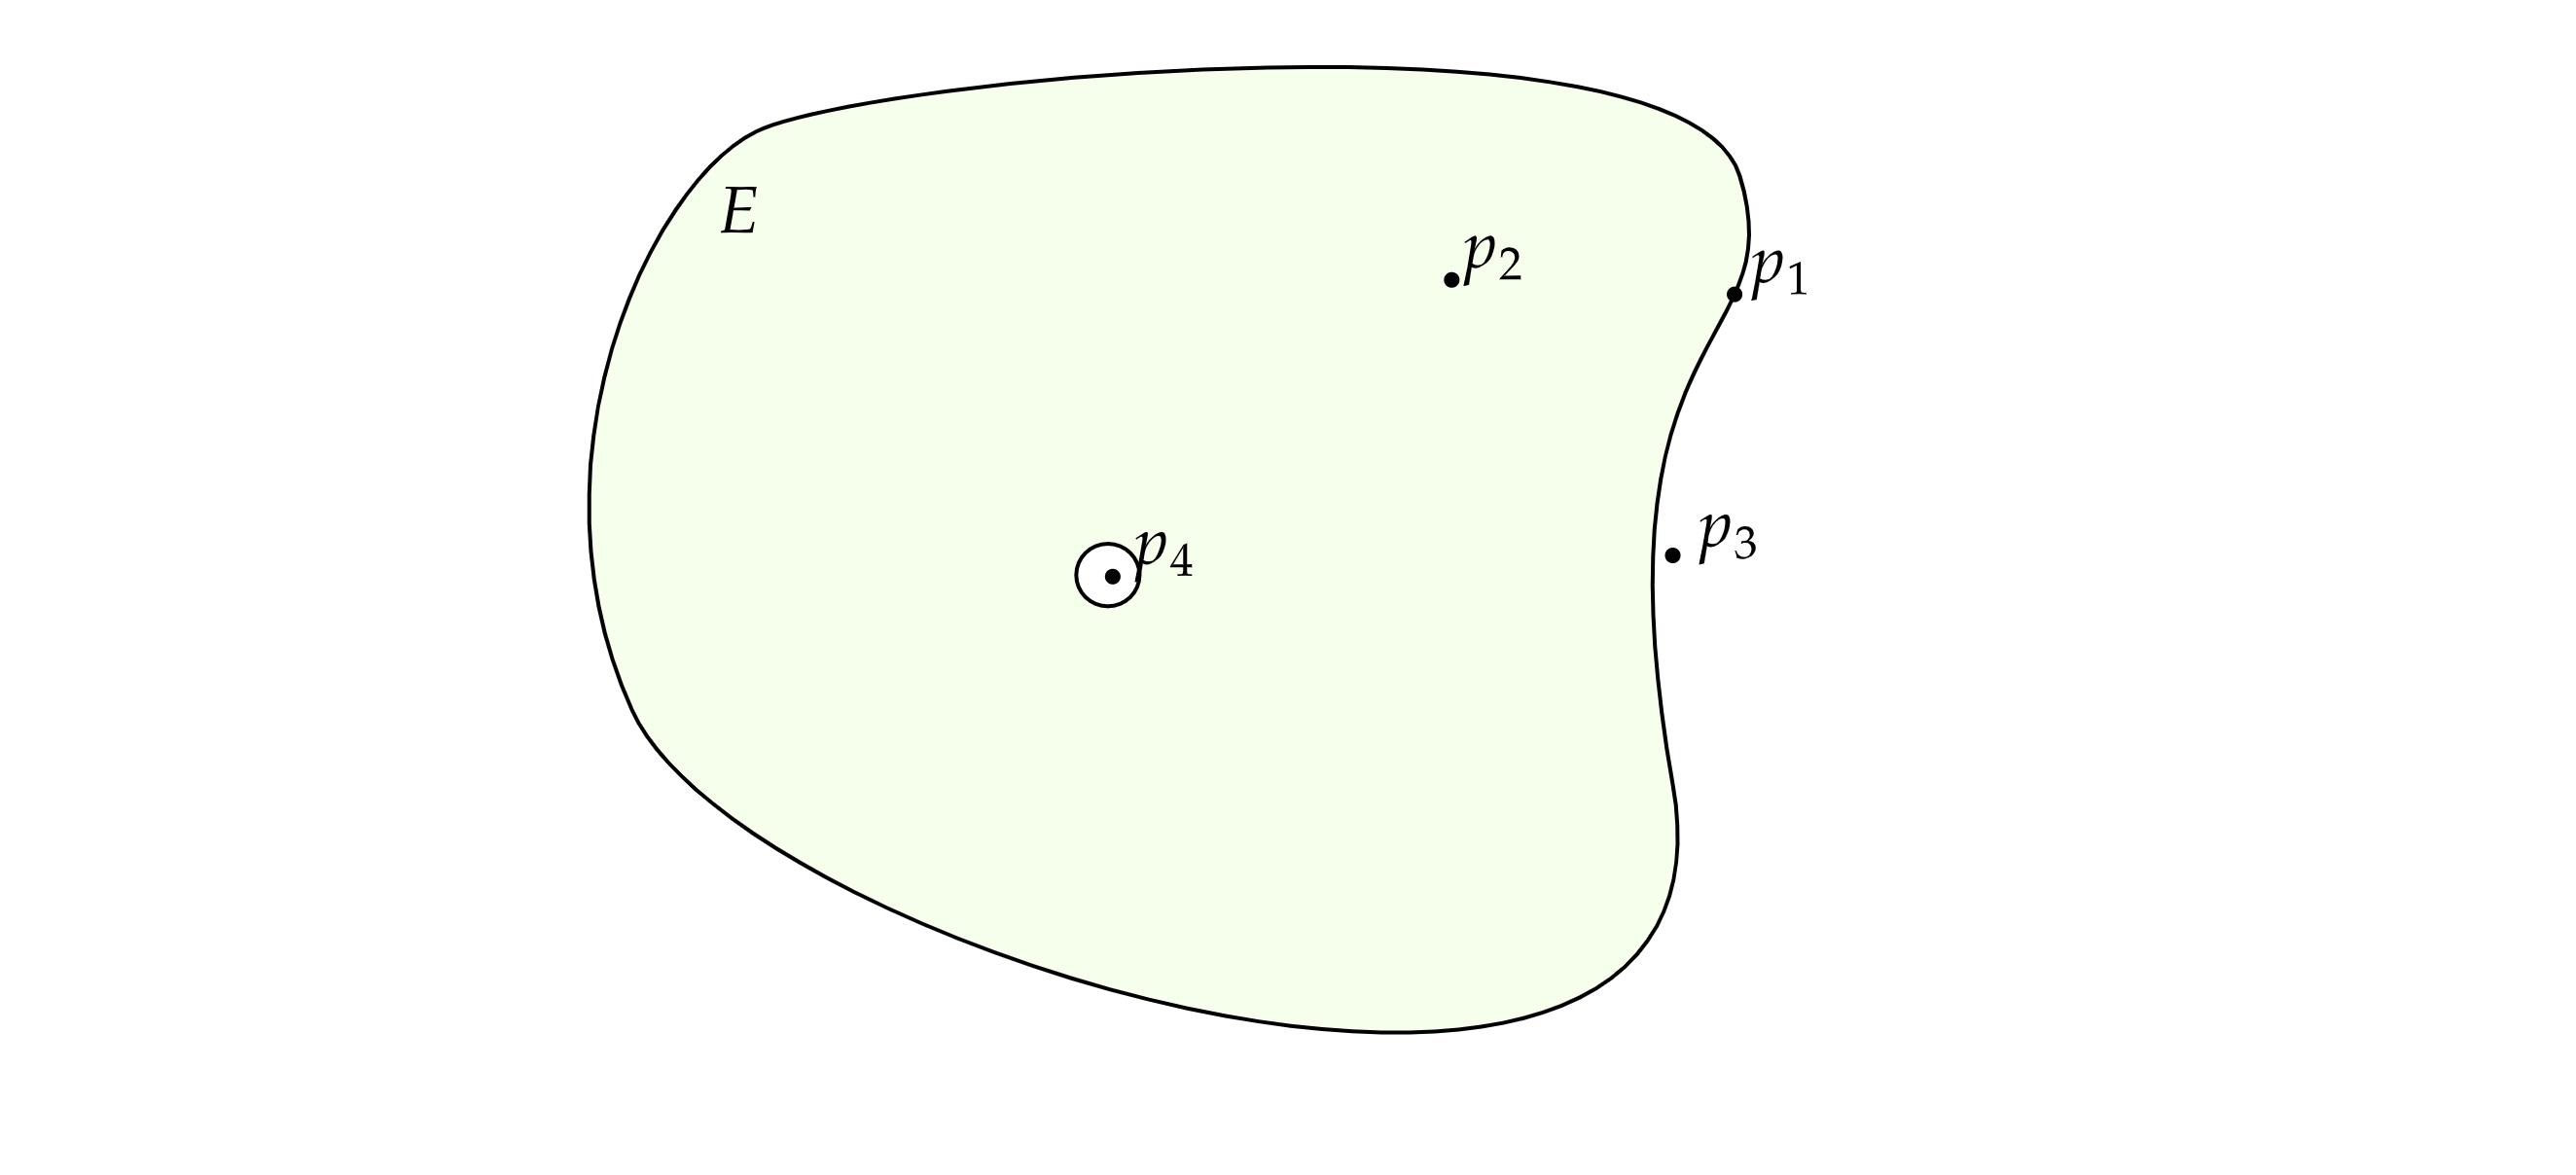
\includegraphics[width=0.8\textwidth]{figures/d1.png}
    \caption{\label{fig:d1.png}
        $p_1$, $p_2$ are limit points; $p_3$, $p_4$ are isolated points. Also, $p_1 \in E$ and $p_1$ is not interior point of $E$ so $E$ is not open. But $E$ is closed.
    }
\end{figure}

\begin{figure}[H] \centering
    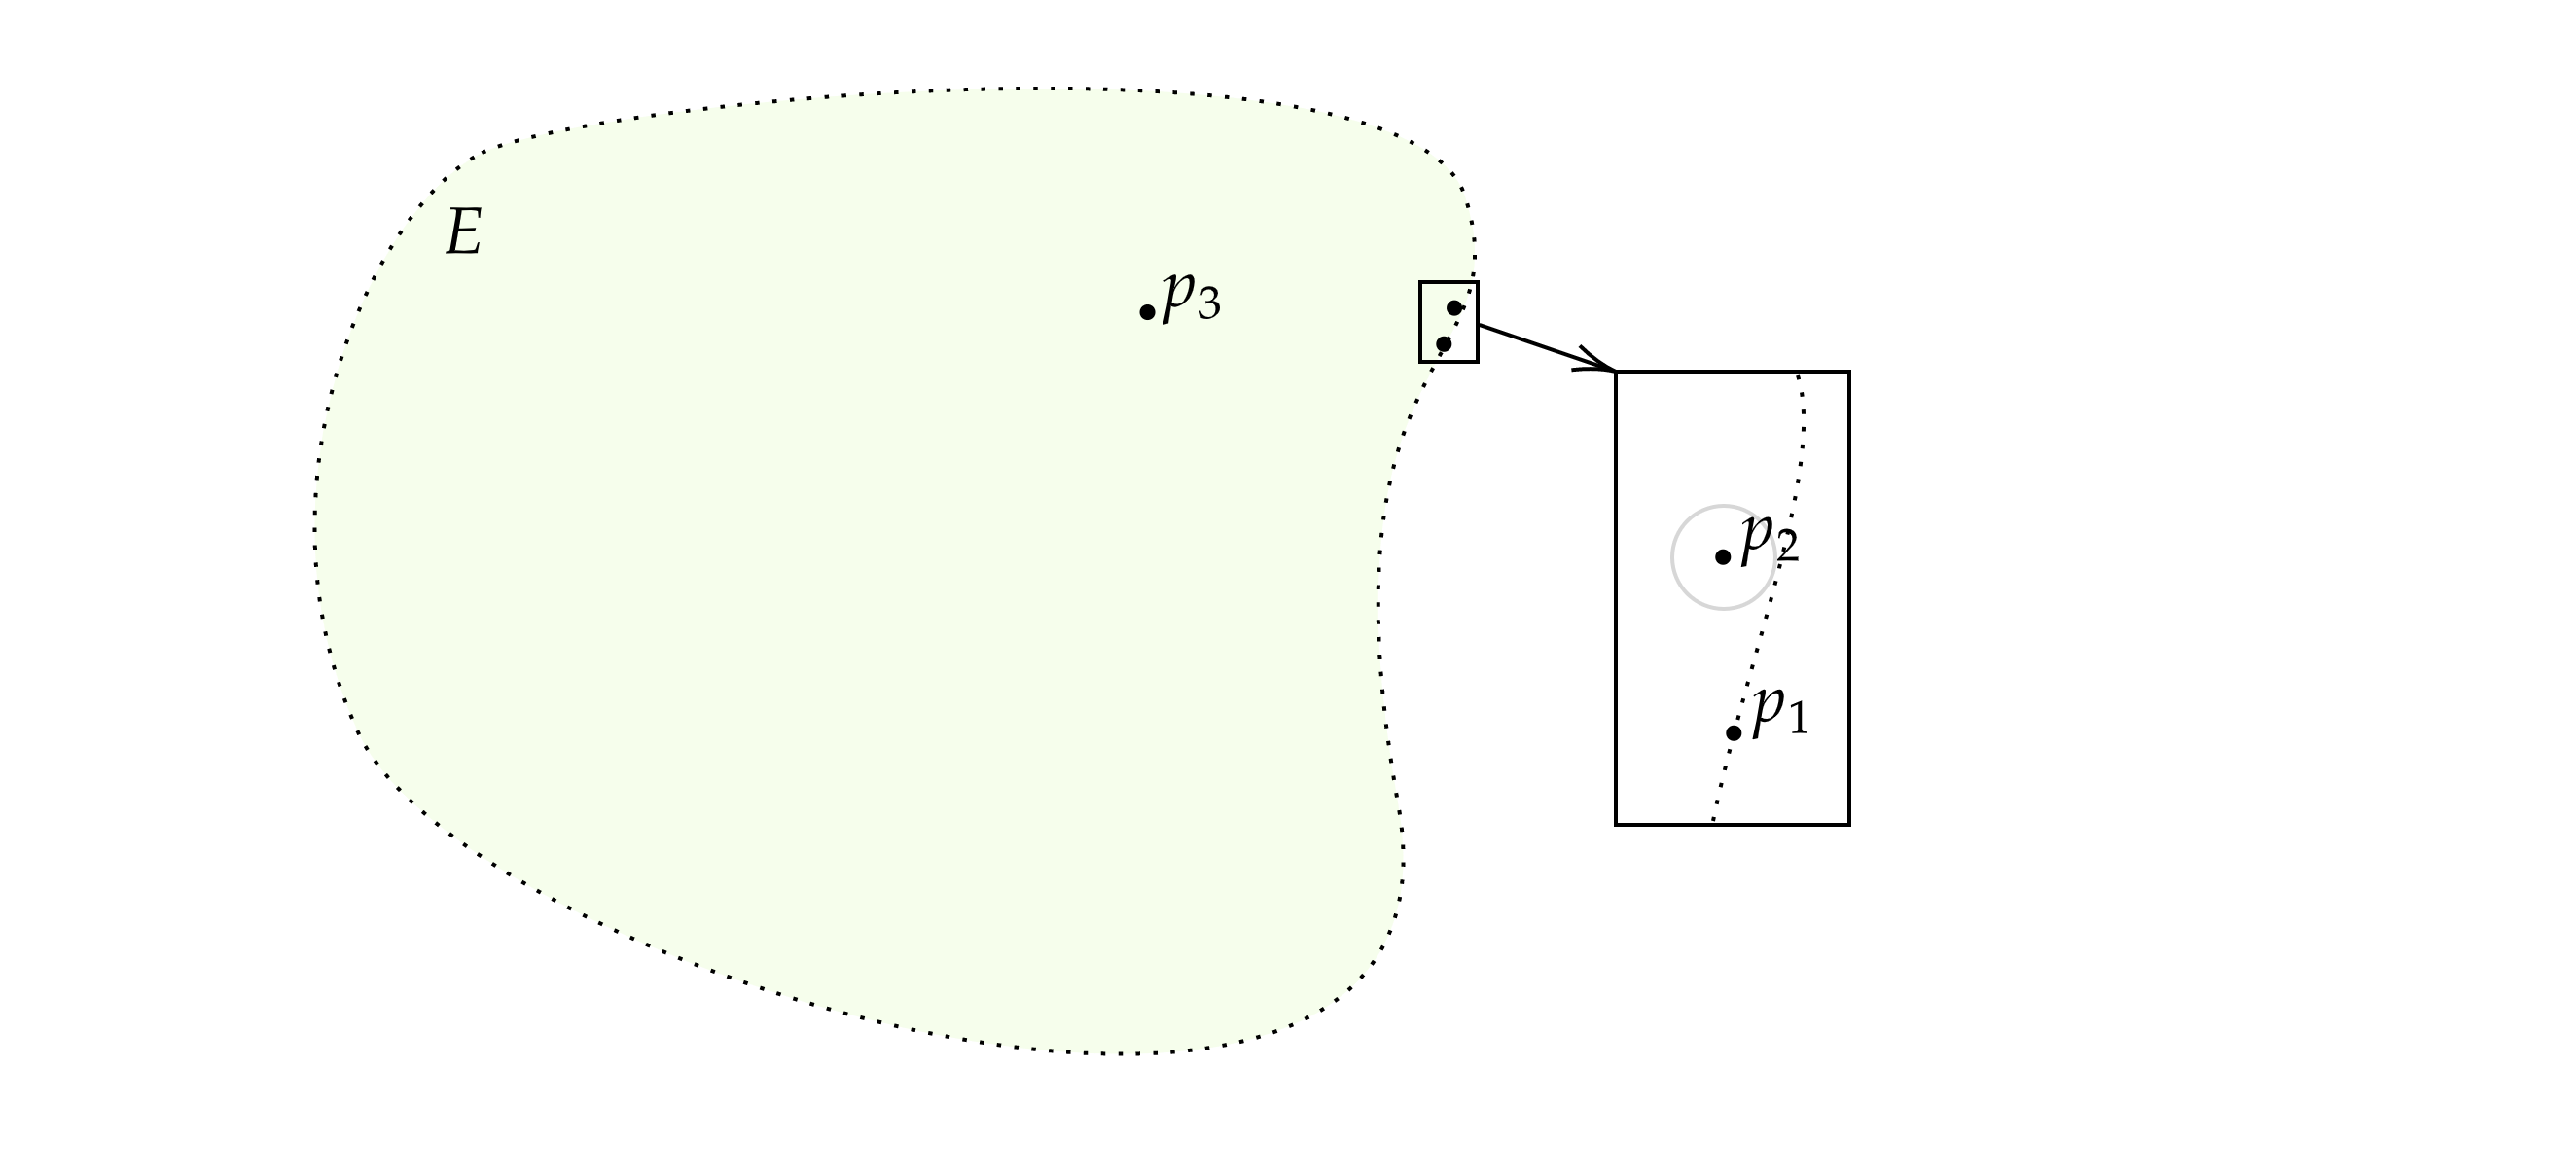
\includegraphics[width=0.8\textwidth]{figures/d2.png}
    \caption{\label{fig:d2.png}
        $p_1$ is a limit point but not in $E$; $p_2$ is an interior point; all three are limit points. $E$ is open but not closed.
    }
\end{figure}

\begin{eg} Let the following be subsets of $\mathbb{R}^{2}$.
    \begin{enumerate}
        \item $\{ z:z \in \mathbb{C}, |z| < 1 \}$
        \item $\{ z:z \in \mathbb{C}, |z| \le  1 \}$
        \item A finite set.
        \item $\mathbb{Z}$
        \item $\{ \frac{1}{n} : n \in \mathbb{N} \}$
        \item $\mathbb{C}$ or $\mathbb{R}^{2}$
        \item The segment $(a,b)$
    \end{enumerate}
    \begin{center}
        \begin{tabular}{|c|*{4}{c|}}
            \hline
             Example &\textbf{Closed} &\textbf{Open} &\textbf{Perfect} &\textbf{Bounded} \\
            \hline
            1 & No &Yes &No &Yes \\ \hline
            2 & Yes &No &Yes &Yes \\ \hline
            3 & Yes &No &No &Yes \\ \hline
            4 & Yes &No &No &No \\ \hline
            5 & No &No &No &Yes \\ \hline
            6 & Yes &Yes &Yes &No \\ \hline
            7 & No & $\dagger$ &No &Yes \\
            \hline
    \end{tabular}
    \\ $\dagger$ Yes if $(a,b) \subset \mathbb{R}$, No if $(a,b) \subset \mathbb{R}^{2}$
    \end{center}
\end{eg}

\begin{definition}[Relatively Open] Let $E \subset Y \subset X$, where $(X,d)$ is a metric space.
\\Then $E$ is \textit{open relative to $Y$} if $E$ is an open set of the metric space $(Y,d)$.
\end{definition}

\begin{remark}
    The segment $(a,b)$ is open relative to $\mathbb{R}$ but not $\mathbb{R}^{2}$.
\end{remark}

\begin{prop} ~
\begin{enumerate}
    \item Every neighborhood is an open set.
    \item If $p$ is a limit point of a set $E$, then every neighborhood of $p$ contains infinitely many points of $E$.
    \subitem 2.1. A finite point set has no limit points.
    \item A set $E$ is open if and only if its complement is closed.
\end{enumerate}
\end{prop}
\begin{proof}
\begin{enumerate} ~
    \item .
    \item .
    \item If $E$ is open, assume $\exists x \in E^{c}$, such that $x$ is a limit point of $E^{c}$ and $x \notin E^{c}$. \\ Then $x \in E$ and $x$ is an interior point in $E$, implies there exists a neighborhood $N$ of $x$, such that $N \subseteq E$, implies $N \not\subseteq E^{c}$, implies that $x$ is not a limit point of $E^{c}$, which contradicts to the assumption. $E^{c}$ is closed. 
    \\If $E^{c}$ is closed, $\forall x \in E$, $x \notin E^{c}$, and $x$ is not a limit point of $E^{c}$, implies there exists a neighbor $N$ of $x$ such that $N \not \subseteq E^{c}$, implies $N \subseteq E$. $E$ is open.
\end{enumerate}
\end{proof}

\begin{prop} ~
\begin{enumerate}
    \item For any collection $\{ G_{\alpha} \}$ of open sets, $\bigcup_{\alpha} G_{\alpha}$ is open.
    \item For any collection $\{ F_{\alpha} \}$ of closed sets, $\bigcap_{\alpha} F_{\alpha}$ is closed.
    \item For any finite collection $\{ G_1, \cdots ,G_n \}$ of open sets, $\bigcap_{i=1}^n G_{i}$ is open.
    \item For any finite collection $\{ F_1, \cdots ,F_n \}$ of closed sets, $\bigcup_{i=1}^n F_{i}$ is closed.
\end{enumerate}
\end{prop}
\begin{proof} ~
\begin{enumerate}
    \item Trivial.
    \item Follow from 1, apply De Morgen's Law and \textbf{Proposition 5}-3.
    \item Trivial.
    \item Follow from 3 as in 2.
\end{enumerate}
\end{proof}

\begin{definition}[Closure] Let $X$ be a metric space.
    \\ Let $E \subset X$, and $E'$ be the set of all limit points of $E$, then the \textit{closure} of $E$ is $\bar{E} = E \cup E'$.
\end{definition}

\begin{prop} Let $X$ be a metric space and $E \subset X$, then
\begin{enumerate}
    \item $\bar{E}$ is closed.
    \item $E = \bar{E} \iff E$ is closed.
    \item $\bar{E} \subset F$ for every closed set $F \subset X$ such that $E \subset F$. ($\bar{E}$ is the smallest closed set containing $E$)
\end{enumerate}
\end{prop}
\begin{proof} ~
\begin{enumerate}
    \item Let $x \in \bar{E}^{c}=E^{c}\cap E'^{c}$. Since $x \notin E$ and is not a limit point of $E$, so there exists a neighbor $N$ of $x$, such that $N \cap E = \varnothing$, implies $N \cap E' = \varnothing$ (check this one using contradiction), implies $N \subset E^{c}\cap E'^{c}$. $\bar{E}^{c}$ is open.
    \item Trivial.
    \item Let $F \subset X$ be closed and $E \subset F$, then $F' \subset F$. Since $E' \subset F'$, so $E' \subset F \implies \bar{E}=E \cup E' \subset F$.
\end{enumerate}
\end{proof}

\begin{prop} Let $E$ be a nonempty subset of $\mathbb{R}$ bounded above.
\\ Then $\sup(E)\in \bar{E}$, and $(E$ is closed$)$ $\implies (\sup(E)\in E)$
\end{prop}

\begin{prop} Let $E \subset Y \subset X$ where $(X,d)$ is a metric space.
\\$E$ is open relative to $Y$ if and only if $\exists G, \text{ s.t.}$ $G$ is open relative to $X$ and $E = G \cap  Y$.
\end{prop}
\begin{proof}
TODO
\end{proof}

\subsection{Compactness in Metric Space} \label{sec:}

\begin{definition}[Open cover]
Let $X$ be a metric space. \\An \textit{open cover of $E \subseteq X$} is $\{ G_{\alpha}\}$, where $G_{\alpha}$ is an open subset of $X$, and $E \subseteq \bigcup_{\alpha}G_{\alpha}$.
\end{definition}

\begin{definition}[Compact]
Let $X$ be a metric space, and $K$ a subset of $X$.
\\ $K$ is \textit{compact} if every open cover of $K$ contains a finite subcover that covers $K$.
\end{definition}

\begin{prop}
Suppose $K \subseteq Y \subseteq X$. Then $K$ is compact relative to $Y$ if and only if $K$ is compact relative to $X$.
\end{prop}





